\documentclass[11pt]{article}

\usepackage[margin=0.85in]{geometry}
\usepackage{amsmath, amssymb}
\usepackage{graphicx}
\usepackage{xcolor}
\usepackage[hidelinks]{hyperref}
\usepackage{caption}
\usepackage[compact]{titlesec}
\captionsetup{font=footnotesize}
\titlespacing*{\section}{0pt}{1.2ex plus 0.3ex}{0.6ex plus 0.2ex}
\setlength{\parskip}{0.35ex}

\definecolor{topblue}{HTML}{1f77b4}
\definecolor{botred}{HTML}{d62728}

\newcommand{\utop}{u_{\mathrm{top}}}
\newcommand{\ubot}{u_{\mathrm{bot}}}
\newcommand{\sgtop}{\sigma_{\mathrm{top}}}
\newcommand{\sgbot}{\sigma_{\mathrm{bot}}}

\title{\vspace{-2.5em}Why \texttt{eos\_widget} \S12b Panel~1 goes \textcolor{topblue}{negative}
and Panel~2 goes \textcolor{botred}{positive}\\[0.3em]
\large A loss/function-surface explanation (it is \emph{not} a bug)}
\author{}
\date{}

\begin{document}
\maketitle
\vspace{-3.5em}

\begin{figure}[t]
  \centering
  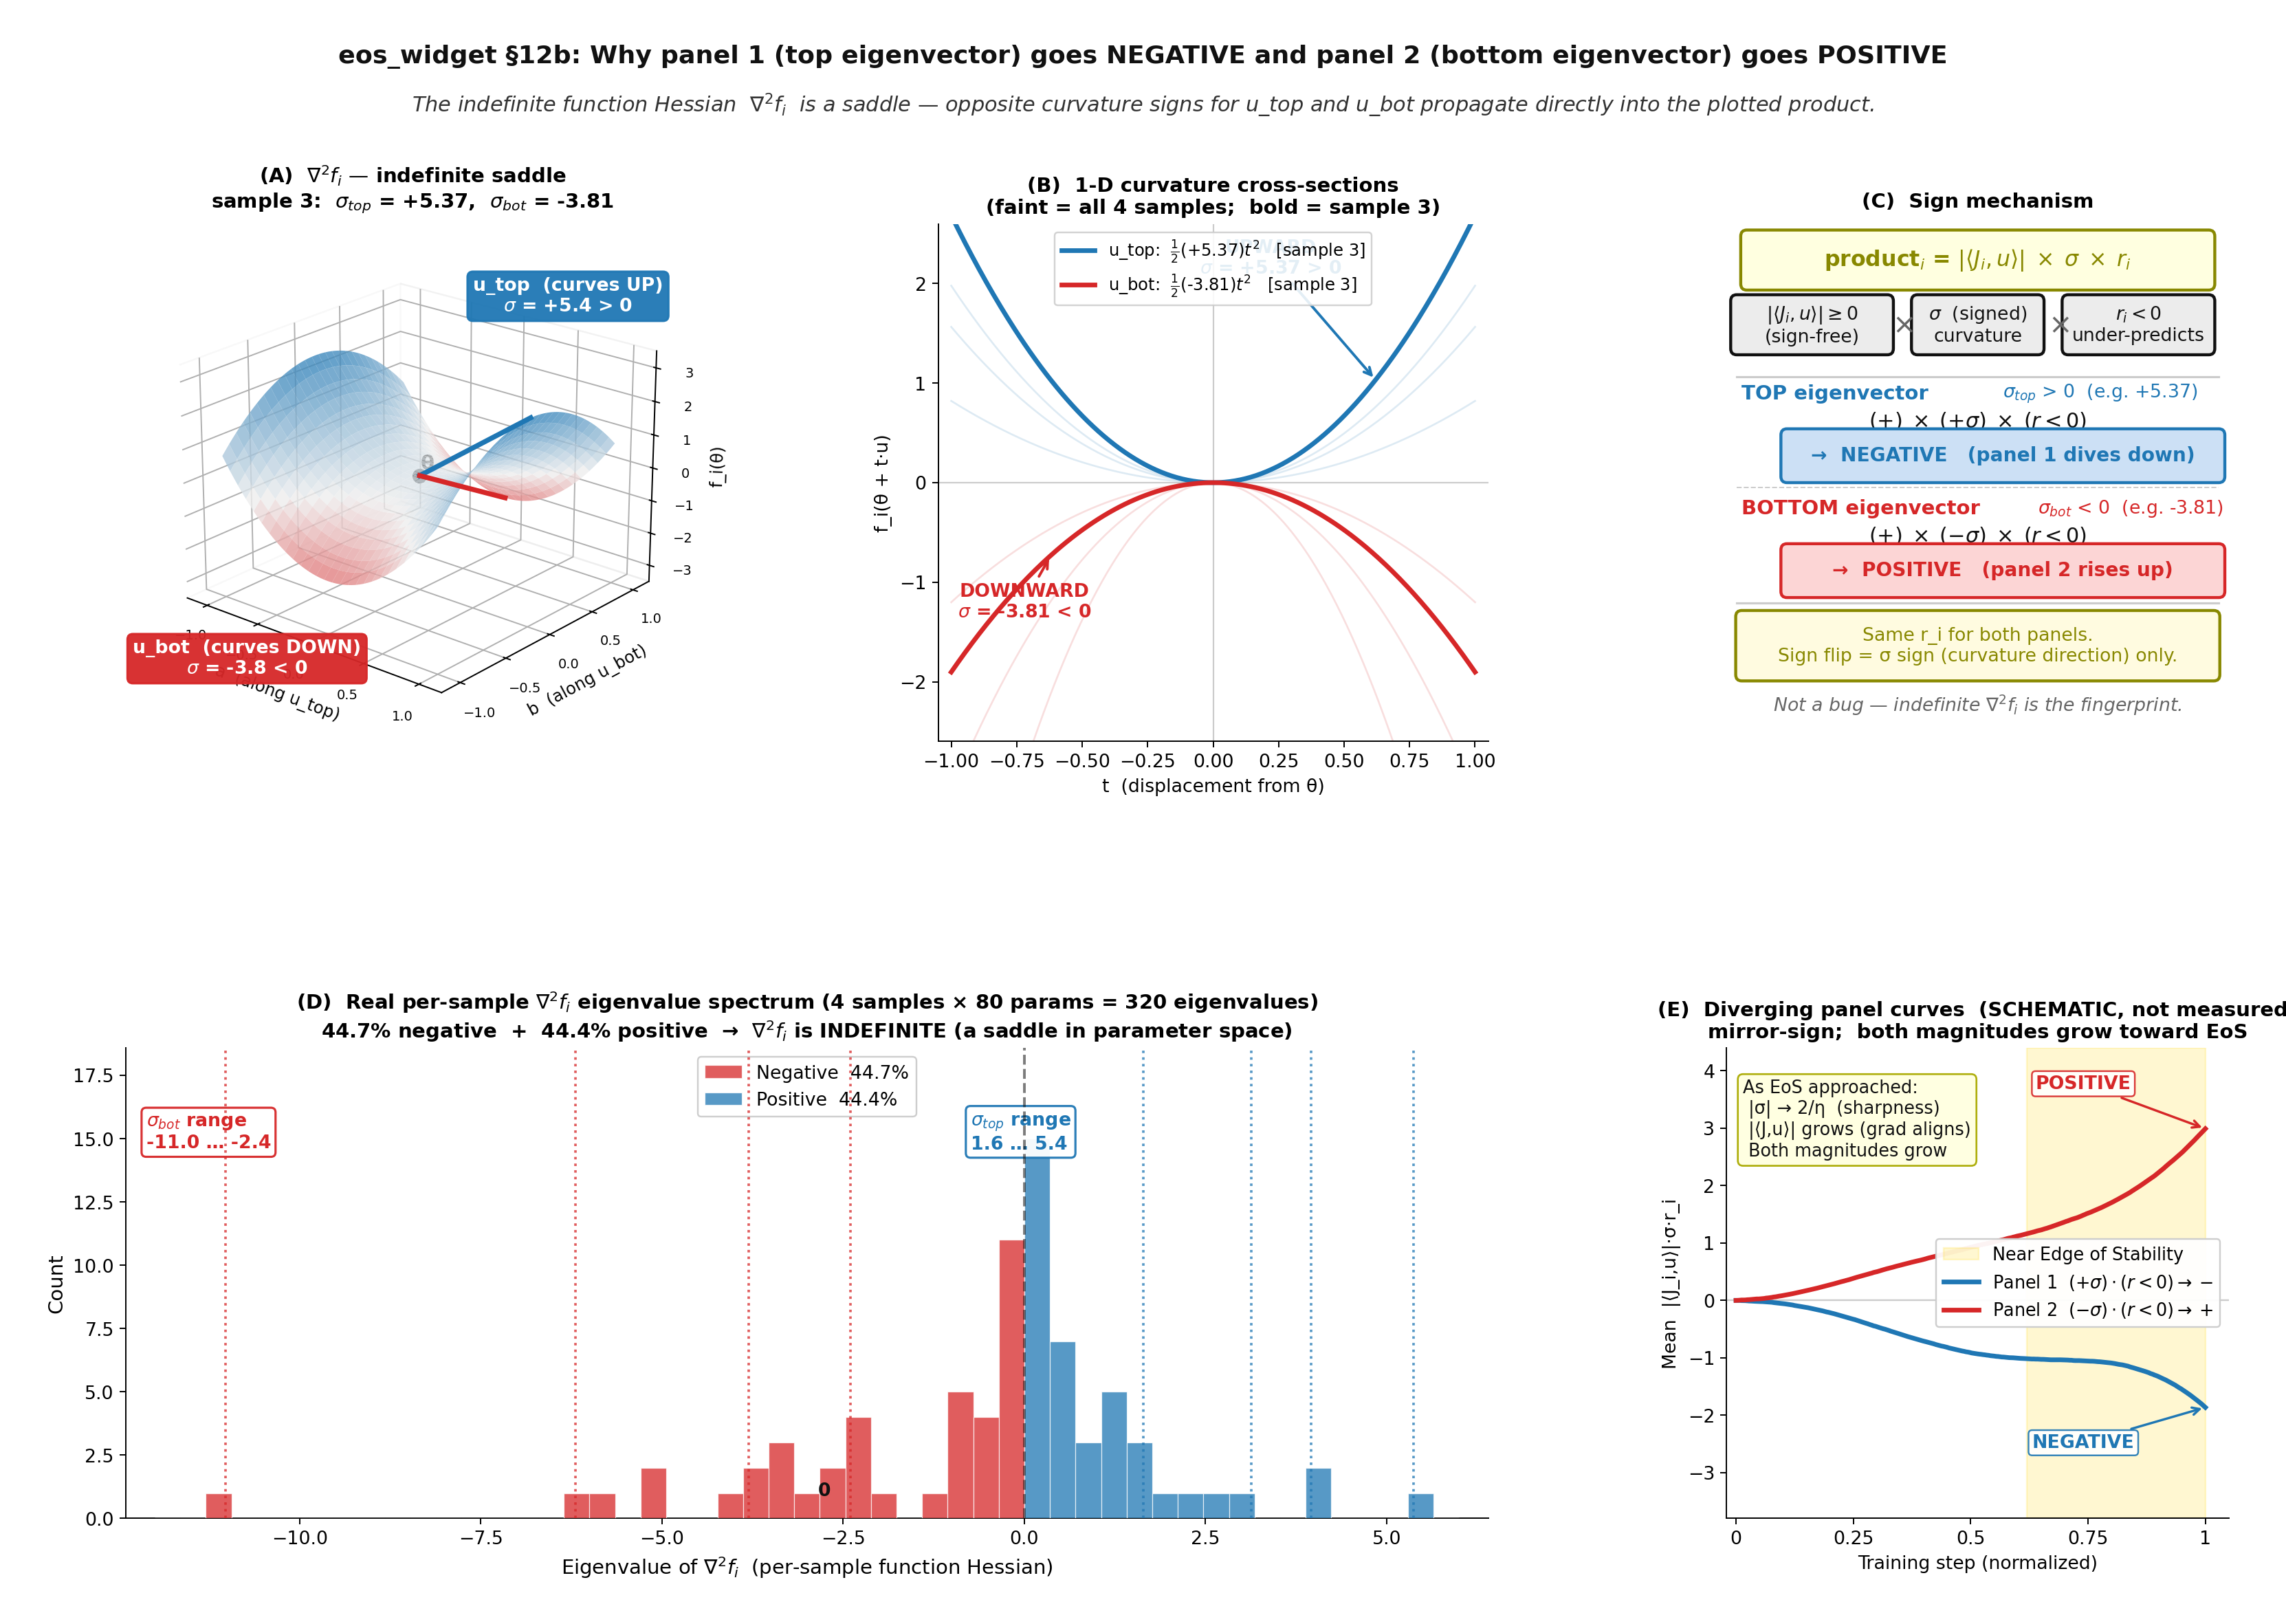
\includegraphics[width=0.74\textwidth]{loss_surface_sign.png}
  \caption{\textbf{The sign split is inherited from the indefinite function Hessian.}
    \textbf{(A)} The per-sample function surface rendered as the indefinite saddle
    $z=\tfrac12(\sgtop a^2+\sgbot b^2)$ with real sample-3 curvatures
    ($\sgtop=+5.37$, $\sgbot=-3.81$): the \textcolor{topblue}{$\utop$} axis curves up
    ($\sigma>0$), the \textcolor{botred}{$\ubot$} axis curves down ($\sigma<0$).
    \textbf{(B)} 1-D cross-sections: an \textcolor{topblue}{upward} parabola along $\utop$ and a
    \textcolor{botred}{downward} parabola along $\ubot$ (faint = all four samples, bold = sample~3).
    \textbf{(C)} The sign mechanism of Eq.~\eqref{eq:product}: the magnitude factor
    $|\langle J_i,u\rangle|\ge0$ is sign-free and the residual $r_i<0$ is shared, so the only
    sign-carrier is $\sigma$. A $+\sigma$ (top) with $r<0$ gives a \emph{negative} product;
    a $-\sigma$ (bottom) with the same $r<0$ gives a \emph{positive} product.
    \textbf{(D)} The real per-sample $\nabla^2 f_i$ eigenvalue spectrum (320 eigenvalues):
    $44.7\%$ negative, $44.4\%$ positive --- it straddles zero, hence indefinite. Dotted lines
    mark each sample's $\sgtop$ (blue) and $\sgbot$ (red).
    \textbf{(E)} Schematic (not measured) of the two diverging panel curves: mirror-sign,
    both magnitudes growing as the Edge of Stability is approached.}
  \label{fig:main}
\end{figure}

\section{What the two panels plot}

The Edge-of-Stability tool's \S12b panels~1 and~2 both plot, as a function of training step,
the per-sample \emph{product}
\begin{equation}
  \mathrm{product}_i \;=\; \bigl|\langle J_i,\, u\rangle\bigr| \;\cdot\; \sigma \;\cdot\; r_i ,
  \label{eq:product}
\end{equation}
averaged over the $N$ samples. Here $J_i = \nabla_\theta f_i$ is the parameter-gradient of the
scalar ground-truth-label logit $f_i(\theta)$, $r_i$ is the per-sample residual, and $(\sigma, u)$
is an eigenpair of the \textbf{per-sample function Hessian} $Q_i = \nabla^2_\theta f_i$ ---
the Hessian of the scalar logit $f_i$ with respect to the network parameters $\theta$
(\emph{not} the loss Hessian, and \emph{not} the Gauss--Newton / GGN operator).
\textbf{Panel~1} uses $u=\utop$, the \emph{top} eigenvector of $Q_i$ (largest eigenvalue
$\sgtop>0$, the direction of maximum upward curvature); \textbf{Panel~2} uses $u=\ubot$, the
\emph{bottom} eigenvector (most-negative eigenvalue $\sgbot<0$, maximum downward curvature).
Both panels multiply by the \emph{same} residual $r_i$, and the magnitude factor
$|\langle J_i,u\rangle|\ge 0$ is sign-free. The observation that Panel~1 drifts increasingly
negative while Panel~2 drifts increasingly positive (both growing in magnitude) is exactly what the
indefinite geometry of $Q_i$ predicts.

\section{The function Hessian is indefinite --- a saddle}

The single fact that explains everything is that $\nabla^2 f_i$ is \textbf{indefinite}: it has both
positive and negative eigenvalues. This is confirmed directly from the real per-sample spectra
(Figure~\ref{fig:main}D): across $4$ samples $\times\, 80$ parameters $=320$ eigenvalues,
\textbf{$44.7\%$ are negative} and \textbf{$44.4\%$ are positive} (the remainder are numerically
zero). The spectrum straddles zero, so $f_i(\theta)$, viewed as a function of the parameters near
the current point, is a \textbf{saddle}, locally
\begin{equation}
  f_i(\theta_0 + a\,\utop + b\,\ubot) \;\approx\;
  f_i(\theta_0) \;+\; \tfrac{1}{2}\bigl(\sgtop\,a^2 + \sgbot\,b^2\bigr),
  \qquad \sgtop>0,\;\; \sgbot<0 .
  \label{eq:saddle}
\end{equation}
Along $\utop$ the surface \emph{curves up} ($\sgtop>0$, an upward parabola); along $\ubot$ it
\emph{curves down} ($\sgbot<0$, a downward parabola). The real extremal eigenvalues are
\begin{equation}
  \sgtop \;\in\; [\,+1.64,\; +5.37\,], \qquad
  \sgbot \;\in\; [\,-11.03,\; -2.40\,].
\end{equation}
Note that $|\sgbot|$ can substantially exceed $|\sgtop|$
($11.03 > 5.37$); this asymmetry is why Panel~2's magnitude tends to \emph{overshoot} Panel~1's.

\section{The sign mechanism}

Decompose Eq.~\eqref{eq:product} into its three factors:
\begin{equation}
  \mathrm{product}_i \;=\;
  \underbrace{\bigl|\langle J_i,u\rangle\bigr|}_{\ge\,0\;\text{(sign-free)}}
  \;\cdot\;
  \underbrace{\sigma}_{\text{signed curvature}}
  \;\cdot\;
  \underbrace{r_i}_{\text{signed residual}} .
\end{equation}
The first factor is an absolute value, hence non-negative. The residual is the \emph{same} $r_i$ in
both panels, and empirically the mean residual is \textbf{predominantly negative} ($r_i<0$): the
model under-predicts the ground-truth-label logit and is being pushed up. With $|\langle J_i,u\rangle|\ge 0$
and $r_i<0$ fixed, the \emph{only} factor that differs between the two panels is the \emph{sign of
$\sigma$}. Therefore
\begin{align}
  \text{\textcolor{topblue}{Panel 1 (top)}:}\quad
    &\bigl|\langle J_i,\utop\rangle\bigr|\,\cdot\,(+\sgtop)\,\cdot\,(r_i<0)
    \;\Longrightarrow\; \textcolor{topblue}{\textbf{NEGATIVE}}, \\[0.2em]
  \text{\textcolor{botred}{Panel 2 (bottom)}:}\quad
    &\bigl|\langle J_i,\ubot\rangle\bigr|\,\cdot\,(-|\sgbot|)\,\cdot\,(r_i<0)
    \;\Longrightarrow\; \textcolor{botred}{\textbf{POSITIVE}} .
\end{align}
The two panels are exact \textbf{mirror images}: the sign is inherited entirely from the curvature
sign of the chosen eigenvector. The factor of $-1$ between $\sgtop>0$ and $\sgbot<0$ propagates
straight through Eq.~\eqref{eq:product}.

\section{Why both magnitudes grow toward the Edge of Stability}

The user's intuition that ``both should increase'' is correct \emph{for the magnitude}; only the
sign differs. As training approaches the Edge of Stability, two effects compound:
(i)~\textbf{progressive sharpening} grows the extremal curvatures, $|\sigma|\to 2/\eta$ (the
sharpness ceiling set by the learning rate $\eta$); and (ii)~\textbf{gradient alignment} rotates
$J_i$ toward the extremal eigenvectors, so $|\langle J_i,u\rangle|$ grows for both $\utop$ and
$\ubot$. Both effects raise $|\mathrm{product}_i|$ in \emph{both} panels, so Panel~1 dives
\emph{more} negative and Panel~2 climbs \emph{more} positive (Figure~\ref{fig:main}E) --- diverging
in sign but growing together in magnitude. Because $|\sgbot|>|\sgtop|$, the bottom panel typically
grows faster.

\section{Conclusion: not a bug}

The opposite directions of the two panels are the \textbf{fingerprint of the indefinite function
Hessian} (a saddle in parameter space), not an error. The chain is:
\begin{equation*}
  \begin{aligned}
  \nabla^2 f_i \text{ indefinite}
    &\;\Rightarrow\; \sgtop>0,\;\sgbot<0 \\
    &\;\Rightarrow\; \text{shared } r_i<0 \text{ flips sign with } \sigma \\
    &\;\Rightarrow\; \text{Panel 1 negative, Panel 2 positive.}
  \end{aligned}
\end{equation*}
For contrast, the \textbf{Gauss--Newton / GGN} operator is positive-semidefinite ($\sigma\ge0$):
if the tool tracked it instead, both ``top'' and ``bottom'' directions would carry a non-negative
$\sigma$ and the two panels \emph{would share a sign}. The observed mirror-image behavior is thus a
direct, expected consequence of choosing the indefinite $\nabla^2 f_i$ as the curvature operator.

\end{document}
